{
	\usebackgroundtemplate{%
		\tikz\node[
			opacity=0.3,
			inner sep=0pt,
		]
		{
			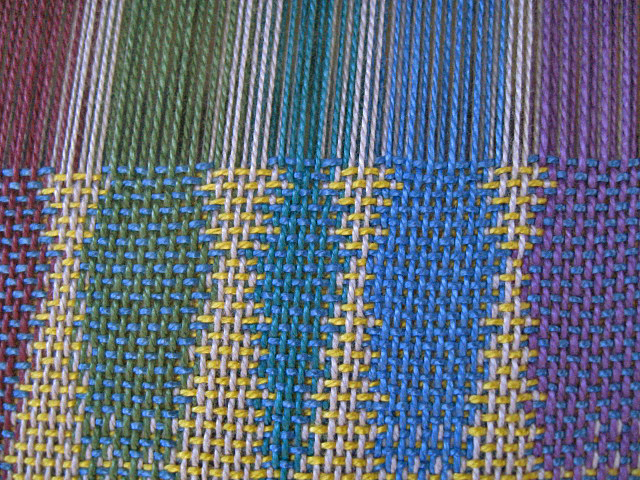
\includegraphics[
				height=\paperheight,
		width=\paperwidth,%
		%opacity=.2%
		]{fig/loom_warp.jpg}%
		};
	}


\begin{frame}
	\frametitle{Hardware implementation}

	\begin{block}{Warps\footnote{``The term \emph{warp} originates from weaving, the first parallel thread technology.''~\cite[p.~69]{cuda:programming}}}
		\begin{itemize}
			\item Are groups of 32 \emph{parallel} threads;
			\item Start at the same program address but each owns an instruction counter and register state so it's free to branch;
			\item Execute \emph{one common instruction at time:} \alert{branches are serialized}.
		\end{itemize}
	\end{block}

	\begin{block}{Streaming Multiprocessors}
		\begin{itemize}
			\item Create, manage, schedule and execute warps;
			\item Run concurrently threads in a block \emph{and} blocks themselves;
			\item Implement no branch prediction nor speculative execution;
			\item \emph{Single Instruction, Multiple Threads:} a single instruction controls all the \cuda{} cores in the multiprocessor.
		\end{itemize}
	\end{block}
%	\gpu{} is built around a scalable array of multithreaded \emph{streaming processors}
\end{frame}
}
